\section{Approximations-Algorithmen}

\begin{takeaway}
    \item Optimierungsproblem, Approximations-Algorithmus, Approximationsgüte
    \item (Metrisches) TSP, Spannbaum-Algorithmus, Christofides
    \item Min-VCP, 2-Approximation
    \item Min-SCP, $\ln(n)$-Approximation (Greedy)
    \item Weighted-VCP, 2-Approximation (LP, Relaxieren)
\end{takeaway}

\paragraph{Definition Optimierungsproblem, Approximationsgüte}
Siehe [ASP].

\paragraph{Travelling Salesperson Problem (TSP)}
Normales und Metrisches TSP ($\Delta$-TSP).
Siehe [ASP].

\paragraph{Spannbaum-Algorithmus für $\Delta$-TSP}
2-Approximation.
Siehe [ASP].

\paragraph{Christofides-Algorithmus}
$\frac{3}{2}$-Approximation.
Siehe [ASP].

\paragraph{Minimum Vertex Cover Problem (Min-VCP)} \mbox{}\\
Eingabe: $G=(V,E)$ \\
Zulässige Lösungen: $C \subseteq V$ so dass jede Kante in $E$ mind. einen Endpunkt in $C$ hat. \\
Kosten: $cost(C) = |C|$ \\
Ziel: min

Intuitiv: Alle Kanten mit mindestens einem Knoten abdecken.

\paragraph{2-Approximation für Min-VCP}
Siehe [ASP].

\paragraph{Set Cover Problem (SCP)} \mbox{} \\
Eingabe: Grundmenge $X$ und Mengensystem $\mathcal{F} \subseteq Pot(X)$ mit $ X = \bigcup_{Q \in \mathcal{F}} Q $ \\
Zulässige Lösungen: $C \subseteq \mathcal{F}$ so dass $ X = \bigcup_{Q \in C} Q $ \\
Kosten: $cost(C) = |C|$ \\
Ziel: min

Intuitiv: alle Grundelemente mit mindestens einem Set abdecken.
Verallgemeinerung von VCP auf Hypergraphen.
\footnote{Aus VCP-Eingabe $G=(V,E)$ konstruiere SCP-Eingabe $(E, \{E_1, ..., E_n\})$
wobei $E_i \subseteq E$ alle Kanten enhält die adjazent zu $v_i \in V$ sind.}

\begin{figure}[h]
    \centering
    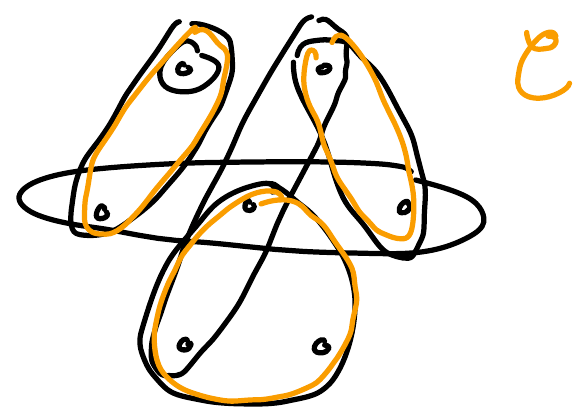
\includegraphics[width=0.3\textwidth]{images/set-cover-problem.png}
    \caption{Beispiel SCP}
\end{figure}

\paragraph{Greedy-Algorithmus für SCP} \mbox{} \\
Eingabe: $(X, \mathcal{F})$
\begin{enumerate}
    \item Initialisierung: $C \gets \emptyset, U \gets X$ \qquad (U = alle noch nicht überdeckten Grundelemente)
    \item while $U \neq \emptyset$ do:
    \begin{itemize}
        \item Wähle $S \in \mathcal{F}$ so dass $|S \cap U|$ maximal
        \item $ U \gets U \setminus S $
        \item $ C \gets C \cup \{ S \} $
    \end{itemize}
\end{enumerate}
Ausgabe: $C$

\paragraph{Theorem}
Greedy-SCP ist ein polynomieller $\ln(n)$-Approximationsalgorithmus für SCP.

\underline{Beweis} (Laufzeit):

Eingabegrösse $n = |X| \cdot |\mathcal{F}|$.
$\min \{|X|, |\mathcal{F}| \} \leq (|X| \cdot |\mathcal{F}|)^{1/2}$ Iterationen
à $\bigO (|X| \cdot |\mathcal{F}|)$
\\
$\implies \bigO ((|X| \cdot |\mathcal{F}|)^{3/2}) = \bigO (n^{3/2})$

\underline{Beweis} (Approximationsgüte):

Schritt 1: Verteile die Kosten von $C$ auf die einzelnen Elemente.

Sei $C = \{ S_1, ..., S_k \}$ die Ausgabe und $S_i$ in Schritt $i$ gewählt.
Sei $D_{C,i} = S_i \setminus \bigcup_{j=1}^{i-1} S_j$ die Differenzmenge,
d.h. die Menge der von $S_i$ neu überdeckten Elemente.

Sei $\forall x \in D_{C,i}$ das $weight_C(x) = \frac{1}{|D_{C,i}|}$
und sei $\forall T \subseteq X$ das $weight_C(T) = \sum_{x \in T} weight_C(x)$.
Beobachte dass (1) $weight_C(D_{C,i}) = 1$ und dass (2) jedes $x \in X$ in genau einem $D_{C,i}$ ist.

$\implies cost(C) = k = \sum_{i=1}^k weight_C(D_{C,i}) = \sum_{x\in X} weight_C(x)$

Schritt 2: Schätze das Gewicht eines beliebigen $S \in \mathcal{F}$ ab.

OBdA sei $S= \{x_1, ..., x_l\}$ so dass $x_j$ bevor oder gemeinsam mit $x_{j+1}$ überdeckt wird. \\
Ziel: $weight_C(x_j) \leq \frac{1}{l-j+1}$.
Beweis per Widerspruch:

Nehme an es gelte für ein $x_j$:
$$ weight_C(x_j) > \frac{1}{l-j+1} \iff |D_{C,i}| = \frac{1}{weight_C(x_j)} < l-j+1 $$
D.h. der Algorithmus überdeckt strikt weniger als $l-j+1$ mit $S_i$ (als er $x_j$ neu überdeckt).
Mit $S$ hätte er aber genau $l-j+1$ (d.h. mehr) Elemente überdecken können.
Widerspruch zu Greedy!

Nun gilt $\forall S \in \mathcal{F}$:
$$ weight_C(S)
     = \sum_{j=1}^l weight_C(x_j)
  \leq \sum_{j=1}^l \frac{1}{l-j+1}
  \leq \sum_{j=1}^l \frac{1}{j}
     = Har(l)
  \leq Har(\max \{ |S| \; | \; S \in \mathcal{F} \} )
$$
wobei $Har$ die Harmonische Zahl ist.

Schliesslich gilt:
\begin{align*}
  cost(C)
     &= \sum_{x \in X} weight_C(x) % see above
  \leq \sum_{S \in C_{Opt}} weight_C(S) % since C_opt ist a set cover
  \leq \sum_{S \in C_{Opt}} Har(\max \{ |S| \; | \; S \in \mathcal{F} \} ) \\
  &\leq |C_{Opt}| \cdot Har(|X|)
  \leq |C_{Opt}| \cdot \ln(n)
\end{align*}
wobei $C_{Opt}$ eine optimale Lösung ist.

$\implies$ Min-SCP $\in$ LOGAPX. Greedy ist optimal für Min-SCP!

\paragraph{Weighted-VCP (WVCP)} \mbox{} \\
Eingabe: $ (G, c)$ wobei $G=(V,E), \; c : V \mapsto \N^+ $ \\
Zulässige Lösungen: jedes vertex cover $C$ von $G$ \\
Kosten: $cost(C) = \sum_{x \in C} c(x)$ \\
Ziel: min

\paragraph{Lineare Programmierung}
LP ist folgendes Optimierungsproblem:
\\
Eingabe: Variablen $(x_1, ..., x_n)^T$,
Konstanten $A^{n \times m} = (a_{ij})_{ij}, \; b = (b_1, ..., b_m)^T, \; c = (c_1, ..., c_n)^T$
\\
Ziel: $\min c^T x = \min \sum c_i \cdot x_i$ unter der Nebenbedingung dass $Ax = b$.

\paragraph{Theorem}
\begin{itemize}
    \item $x_i \in \R$ (LP) $\implies$ in P
    \item $x_i \in \Z$ (Ganzzahl/Integer LP, ILP) $\implies$ NP-schwer
    \item $x_i \in \{0,1\}$ (0/1-LP) $\implies$ NP-schwer
\end{itemize}

\paragraph{WVCP als LP}
\underline{Als 0/1-LP:}
minimiere $\sum c(v_i) \cdot x_i$ \quad unter den Nebenbedingungen:
\begin{itemize}
    \item $\forall \{r,s\} \in E : \; x_r + x_s \geq 1$
    \item $\forall j \in [1,n] : \quad x_j \in \{0,1\}$
\end{itemize}
Intuitiv: $x_j = 1$ falls $v_i \in C$.

\underline{Relaxiere zu LP:}
Ersetze $x_j \in \{0,1\}$ durch $x_j \geq 0$.

\paragraph{Algorithmus LP-VC für WVCP} \mbox{} \\
Eingabe: $I=(G, c)$
\begin{enumerate}
    \item Stelle $I$ als $I_{0/1-LP}(I)$ dar und relaxiere zu $I_{LP}(I)$.
    \item Löse $I_{LP}(I)$. Sei $x = (x_1, ..., x_n), x_i \in \R^+$ die gefundene optimale Lösung.
    \item Setze $C = \{ v_i \st x_i \geq \frac{1}{2} \}$
\end{enumerate}
Ausgabe: $C$

\paragraph{Theorem}
LP-VC ist eine 2-Approximation für WVCP.

\underline{Beweis:}

Laufzeit: offensichtlich.

Korrektheit: $x_r + x_s \geq 1 \implies x_r \geq \frac{1}{2} \vee x_s \geq \frac{1}{2}
\implies v_r \in C \vee v_s \in C \implies \{r, s\}$ abgedeckt

Approximationsgüte:
Beachte dass: $ Opt_{WVCP}(I) = Opt_{0/1-LP}(I_{0/1-LP}(I)) \geq Opt_{LP}(I_{LP}(I)) $. \\
Es gilt:
$$ cost(C)
     = \sum_{v \in C} c(v)
     = \sum_{x_i \geq \frac{1}{2}} c(v_i)
  \leq \sum_{x_i \geq \frac{1}{2}} \underbrace{2 \cdot x_i}_{\geq 1} \cdot c(v_i)
  \leq 2 \cdot \sum_{i=1}^n x_i \cdot c(v_i)
     = 2 \cdot Opt_{LP}(I_{LP}(I))
  \leq 2 \cdot Opt_{WCP}(I)
$$
